\subsection{External interface requirements}
\subsubsection{User interfaces}
\begin{@empty}
The following mockups show an approximation of the mobile application.\\

\setlength{\intextsep}{0pt plus \textheight minus 10pt}

\begin{figure}[H]
\centering
\begin{minipage}{.4\textwidth}
    \centering
    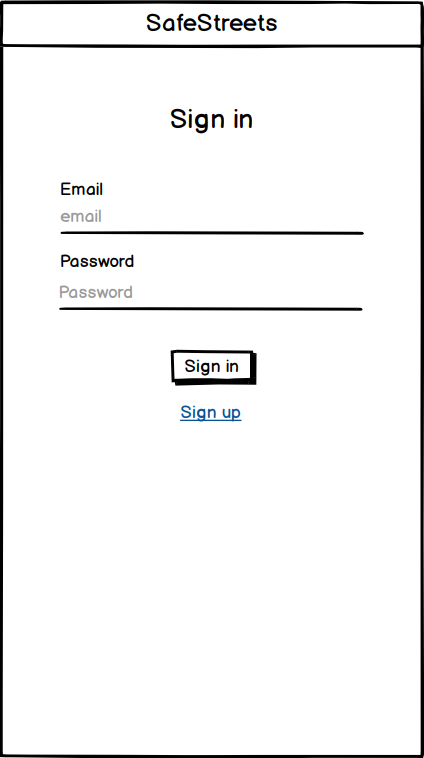
\includegraphics[width=.8\textwidth]{Images/sign-in.png}
    \caption{\label{fig:mockup-sign-in}Mockup - Sign in.}
\end{minipage}
\begin{minipage}{.4\textwidth}
    \centering
    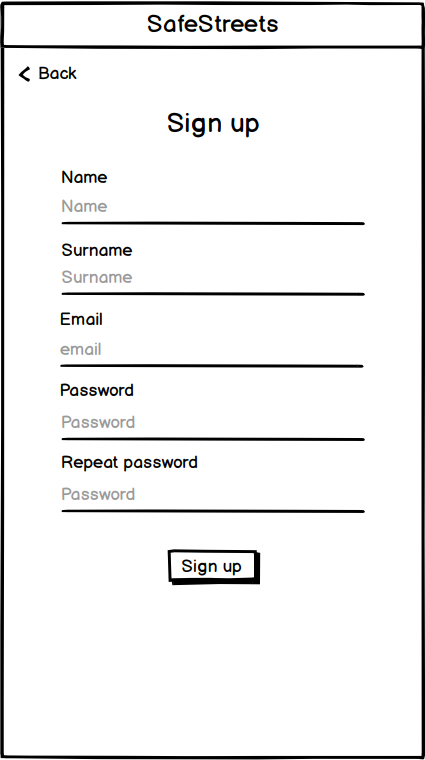
\includegraphics[width=.8\textwidth]{Images/sign-up.png}
    \caption{\label{fig:mockup-sign-up}Mockup - Sign up.}
\end{minipage}
\end{figure}

\begin{figure}[H]
\centering
\begin{minipage}{.4\textwidth}
    \centering
    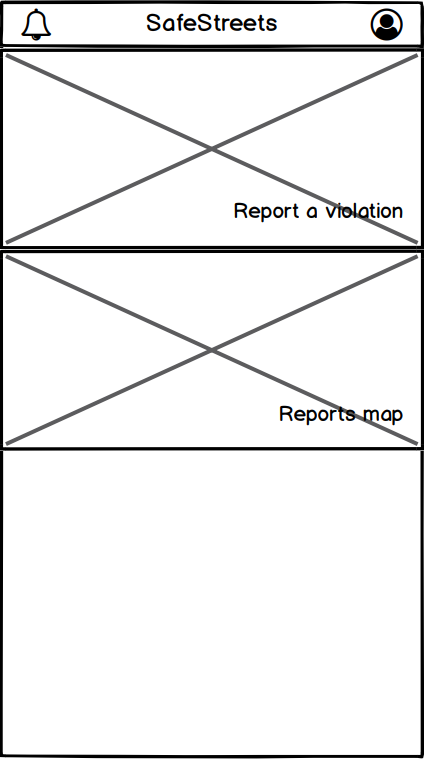
\includegraphics[width=.8\textwidth]{Images/home.png}
    \caption{\label{fig:mockup-home}Mockup - Home.}
\end{minipage}
\begin{minipage}{.4\textwidth}
    \centering
    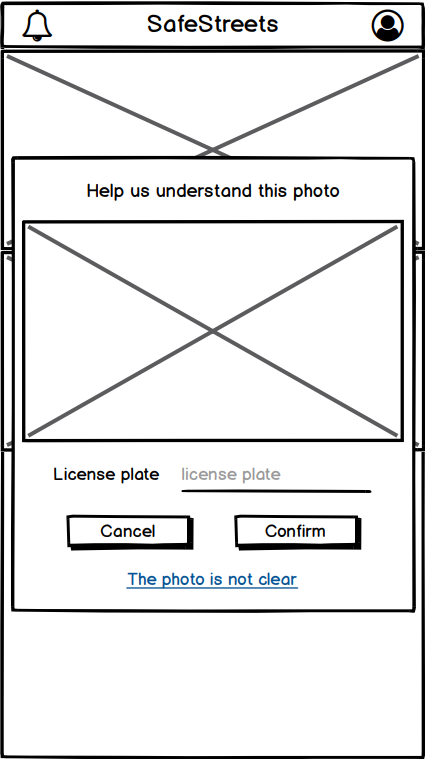
\includegraphics[width=.8\textwidth]{Images/photo-review.png}
    \caption{\label{fig:mockup-photo-review}Mockup - Photo review.}
\end{minipage}
\end{figure}

\begin{figure}[H]
\centering
\begin{minipage}{.4\textwidth}
    \centering
    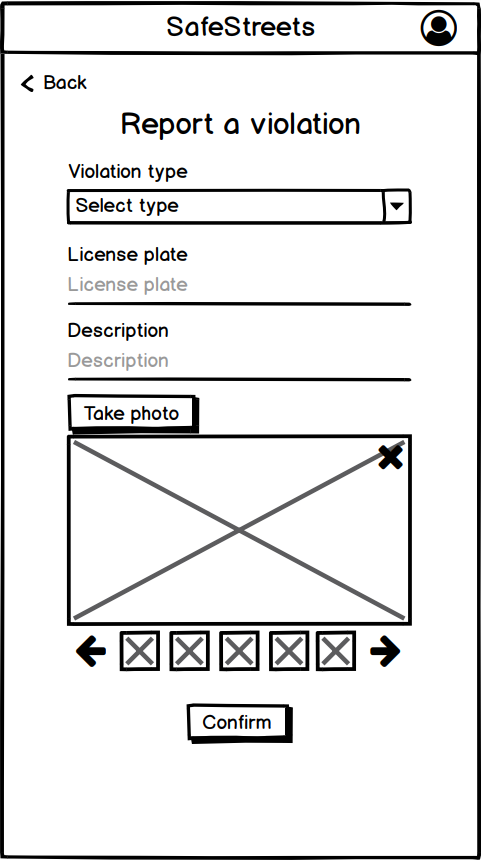
\includegraphics[width=.8\textwidth]{Images/report-violation.png}
    \caption{\label{fig:mockup-report-violation}Mockup - Report violation.}
\end{minipage}
\begin{minipage}{.4\textwidth}
    \centering
    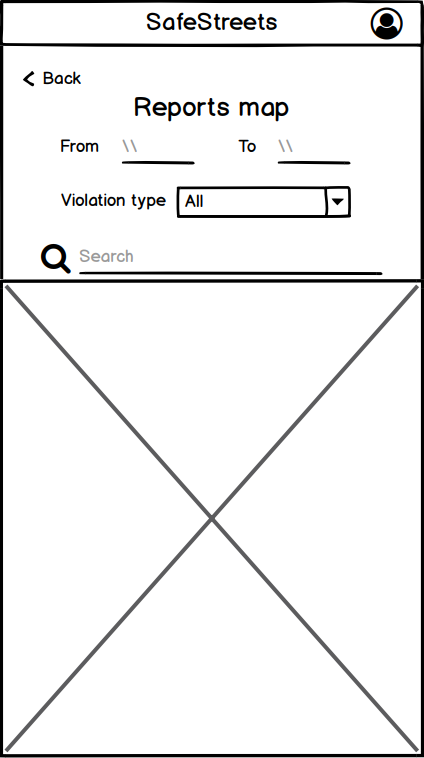
\includegraphics[width=.8\textwidth]{Images/reports-map.png}
    \caption{\label{fig:mockup-reports-map}Mockup - Reports map.}
\end{minipage}
\end{figure}
\end{@empty}

\subsubsection{Hardware interfaces}
\subsubsection{Software interfaces}
\begin{itemize}
\item
License plate recognition: it is necessary to be able to recognize the license plate in the picture a report. For this, a good option is OpenALPR, an open source library that can be run server-side (due to performance limitations). A cloud API is also provided, which could be used during early stages of development.
\end{itemize}
\subsubsection{Communication interfaces}

\subsection{Scenarios}
\subsubsection{Scenario 1}
John has a spot on his street reserved for his garage entrance. During the week, he commutes to work by subway, and leaves the car to his wife, Sarah, who leaves later in the day. It is not unusual for him to find someone blocking the garage when he goes to work in the morning. If the car is still there by the time Sarah needs to leave, she will be late to the office. 
Before using SafeStreets, he would have to call the police and provide a license plate and address, all while hurrying on his way to work. Now, he can just take a picture and then submit a report while he is sitting on the subway.
\subsubsection{Scenario 2}
Marco is a data science student at Politecnico di Milano. As he bikes every day to the university, he is familiar with the problem of cars parking in the bike lane. Thanks to the SafeStreets API, he can easily obtain data about it using Python. So, he decides to base his thesis on this topic and analyzes the patterns in violations throughout all of Italy, comparing different cities and their countermeasures.
\subsubsection{Scenario 3}
Chad’s girlfriend broke up with him last week because he was too jealous and would not let her go out with her friends. He is not over this and is really mad at her. All of the sudden he gets a brilliant idea, he takes a picture of the license plate of the girls car and prints it. Then, a couple days later he finds a double parked car, attaches the printed license plate to it and reports the incident with SafeStreets. 
The system detects that something is wrong with the picture, so it decides not to save the report and marks Chad’s account with potential misuse of the application.
\subsubsection{Scenario 4}
Sally wants to go to the city centre to buy some groceries, but she is not sure if she should take the car or go by bus. She grabs her phone, boots up SafeStreets and checks the vicinity to the supermarket. The app shows a high concentration of badly parked cars, she assumes that there is a lot of traffic and nowhere to park her car properly, so she decides to take the bus.

\subsection{Functional requirements}
\begin{itemize}
\item
[G1] - The user is able to report a traffic violation to authorities
    \begin{itemize}
    \item
    D1 - An accurate gps location can be acquired from the device the user is running SafeStreets on.
    \item
    D2 - The device running SafeStreets has a camera.
    \item
    D4 - The metadata of the picture in the violation report is accurate
    \item
    R1 - The user must be able to fill out a form providing information about a traffic violation.
    \end{itemize}

\item
[G2] - License plates can be recognized from the pictures of the violation report
    \begin{itemize}
    \item
    \end{itemize}

\item
[G3] - Roles with different levels of permission are assigned to users and authorities.
    \begin{itemize}
    \item
    \end{itemize}
\item
[G4] - The information gathered from the reports is provided to users and authorities according to their role.
    \begin{itemize}
    \item
    \end{itemize}

\item
[G5] - The system must protect the chain of custody of the reports 
    \begin{itemize}
    \item
	RX - The system must provide e2e encryption from the device of the user to the server.
    \end{itemize}
	
\item
[G6] - Reports that had their integrity compromised and malicious reports will be detected and discarded.
    \begin{itemize}
    \item
	D5 - There is a system available capable of connecting a license plate to characteristics of the car (make, model, color).
    \item
	RX - SafeStreets must cross reference the information of the car registered under the detected license plate with the information obtained from analyzing the report picture.
    \end{itemize}
\item
[G7] - Information about issued tickets provided by the municipality system can be cross referenced with the SafeStreets database and analysed 
    \begin{itemize}
    \item
    \end{itemize} 
 \end{itemize}

\subsubsection{Use cases}

% CASE 1: SIGN UP
\begin{table}[H]
\begin{tabular}{|p{0.17\linewidth}|p{0.77\linewidth}|}
\hline
Name            & Sign up
\\ \hline

Actor           & User
\\ \hline

Entry condition &
- The user has installed the application on their device.

- The application is running.
\\ \hline
%Event flow      & \begin{tabular}[c]{p{0.95\linewidth}}
Event flow      & 
    1. The user presses the “Sign up” button.

    2. The user fills the fields with the required data.

    3. The user presses the “Confirm” button.

    4. The system saves the data.
%\end{tabular}
\\ \hline
Exit condition  & 
 - The user is successfully registered in the system.

 - The user is redirected to the login screen.
\\ \hline
Exceptions      &
    - The user is already registered in the system. The system warns the user that the email is already in use. 

    - The user did not fill all the required fields. The system marks the empty fields for the user to fill.

    - The password does not meet the security requirements. The system asks the user to enter another password.
\\ \hline
\end{tabular}
\end{table}

% CASE 2: SIGN IN 
\begin{table}[H]
\begin{tabular}{|p{0.17\linewidth}|p{0.77\linewidth}|}
\hline
Name            & Sign in
\\ \hline

Actor           & User
\\ \hline

Entry condition &
- The application is running.

- The user is signed up.
\\ \hline
Event flow      & 
    1. The user presses the “Sign in” button.

    2. The user fills the “Username” and “Password” fields.

    3. The user presses the “Sign in” button.
    
    4. The system verifies the user credentials.
\\ \hline
Exit condition  & 
    - The user is successfully signed into the system.

    - The user is redirected to the home screen.
\\ \hline
Exceptions      &
    - The user enters a non matching combination of “username” and “password”. The system shows a warning that “username” and “password” do not match.

    - The user did not fill all the required fields. The system marks the empty fields for the user to fill.
\\ \hline
\end{tabular}
\end{table}

% CASE 3: SEE PROFILE 
\begin{table}[H]
\begin{tabular}{|p{0.17\linewidth}|p{0.77\linewidth}|}
\hline
Name            & See profile
\\ \hline

Actor           & User
\\ \hline

Entry condition &
- The application is running.

- The user is signed in.

- The user is in the home screen.
\\ \hline
Event flow      & 
    1. The user presses the user icon button.

    2. The system shows the user information.
\\ \hline
Exit condition  & 
    - The user information is displayed to the user.
\\ \hline
\end{tabular}
\end{table}

% CASE 4: EDIT USER INFORMATION 
\begin{table}[H]
\begin{tabular}{|p{0.17\linewidth}|p{0.77\linewidth}|}
\hline
Name            & Edit user information
\\ \hline

Actor           & User
\\ \hline

Entry condition &
- The application is running.

- The user is signed in.

- The user is in the home screen.
\\ \hline
Event flow      & 
    1. The user presses the “edit” button.

    2. The user edits the fields they want to change.

    3. The user presses the “confirm” button.
    
    4. The system saves the data.
\\ \hline
Exit condition  & 
    - The user information is successfully updated.

    - The user profile is in view-only state.
\\ \hline
Exceptions      &
    - The user did not fill all the required fields. The system marks the empty fields for the user to fill.

    - The email is already registered in the system. The system warns the user that the email is already in use.
\\ \hline
\end{tabular}
\end{table}

% CASE 5: SUBMIT REPORT 
\begin{table}[H]
\begin{tabular}{|p{0.17\linewidth}|p{0.77\linewidth}|}
\hline
Name            & Submit report
\\ \hline

Actor           & User
\\ \hline

Entry condition &
    - The application is running.

    - The user is signed in.

    - The user is in the home screen.

    - The user’s GPS is active.
\\ \hline
Event flow      & 
    1. The user presses the “Report a violation” button.

    2. The user fills the fields with the required data.

    3. The user presses the “Take photo” button.

    4. The user takes a photo of the vehicle committing the violation.

    5. The user repeats steps 3 and 4 as desired until the amount of photos reaches the limit.

    6. The user presses the “Confirm” button.

    7. The system prompts the user to select a photo where the license plate is clearly identifiable.

    8. The user selects a photo.

    9. The user presses the “Confirm” button.
    
    10. The system submits the report
\\ \hline
Exit condition  & 
    - The report is successfully submitted.
\\ \hline
Exceptions      &
    - The user did not fill all the required fields. The system marks the empty fields for the user to fill.

    - The user did not take a photo. The system warns the user to take a photo
\\ \hline
\end{tabular}
\end{table}

% CASE 6: SEE REPORTS MAP 
\begin{table}[H]
\begin{tabular}{|p{0.17\linewidth}|p{0.77\linewidth}|}
\hline
Name            & See reports map
\\ \hline

Actor           & User
\\ \hline

Entry condition &
    - The application is running.

    - The user is signed in.

    - The user is in the home screen.
\\ \hline
Event flow      & 
    1. The user presses the “Reports map” button.

    2. The user fills the “from”, “to” and “type” fields.

    3. The user presses the “filter” button.

    4. The system shows an interactable map with reports that match the filter.
\\ \hline
Exit condition  & 
    - The system shows the reports map.
\\ \hline
Exceptions      &
    - No reports matching the filter were found. The system shows the empty map.
\\ \hline
\end{tabular}
\end{table}

% CASE 7: REVIEW PHOTO 
\begin{table}[H]
\begin{tabular}{|p{0.17\linewidth}|p{0.77\linewidth}|}
\hline
Name            & Review photo
\\ \hline

Actor           & User
\\ \hline

Entry condition &
    - The application is running.

    - The user is signed in.

    - The user is in the home screen.
\\ \hline
Event flow      & 
    1. The user presses the review photo button.

    2. The user fills the “license plate” field.

    3. The user presses the “confirm” button.

    4. The system saves the review.
\\ \hline
Exit condition  & 
    - The review is saved in the system.

    - The system shows another photo to review.
\\ \hline
Exceptions      &
    - The user did not fill the “license plate” field. The system marks the empty field for the user to fill.
    - The user presses the “The photo is not clear” button. The system shows another photo to review.
\\ \hline
\end{tabular}
\end{table}

\subsection{Performance requirements}

\subsection{Design constraints}

\subsubsection{Standards compliance}

\subsubsection{Hardware limitations}

For use of the mobile application, a smartphone or tablet with the following specifications is required:
\begin{itemize}
   \item 
    Internet connection (Wi-Fi/4G/3G/2G)
   \item 
    GPS
   \item 
    Camera
   \item 
    Android or iOS operating system
\end{itemize}


\subsection{Software system attributes}
\subsubsection{Reliability}
The application is expected to run continuously with no downtime. But given that the system is by no means critical to any of its users, exceptions to this requirement are tolerated. In terms of stored data, the system is required to be fault tolerant, which means that the data needs to be replicated and stored in more than one location.

\subsubsection{Availability}
Although minimal downtime is tolerated, the system is expected to be available 99.9\% of the time. Because of this, some redundancy is to be provided in the application servers.

\subsubsection{Security}
The system manages sensitive user data, which requires confidentiality. Information like passwords is encrypted before being stored in the database.
Measures are to be taken for the protection of servers and databases from both external attacks and hardware malfunctions.


\subsubsection{Maintainability}
The application is meant to be continuously worked and improved upon, possibly by different teams. This means that good design and documentation are required to facilitate its maintainability.

\subsubsection{Interoperability}
The system both utilizes services provided by other systems and acts as a service provider. It needs to be compliant with standards for information exchange between systems and provide a clear interface for external users.
